\documentclass[10pt,a4paper,twocolumn]{article}
\usepackage[margin=2cm]{geometry}
\usepackage{amsmath}
\usepackage{graphicx}
\usepackage{booktabs}
\usepackage{tabularx}
\usepackage{algorithm}
\usepackage{algpseudocode}
\usepackage{xcolor}
\usepackage{hyperref}

\graphicspath{{../figures/generated/}{../figures/}}

% Every \todo{} is something only you can fill in. Search for "todo" before submitting.
\newcommand{\todo}[1]{\textcolor{red}{[TODO: #1]}}

\title{On-Device Light-Condition Classification with a 1\,KB Density Lookup Table:\\
A Proof of Concept on the ESP32-S3}
\author{Vincent Forget\\Project I -- Proposal, Planning \& Prototyping (247-519-VA)\\Vanier College}
\date{\todo{Submission date}}

\begin{document}
\maketitle

\begin{abstract}
The previous lab proposed a pipeline of DBSCAN, per-class kernel density estimation,
a $G\times G$ byte table, and a lookup table, and supported it with synthetic data.
This report tests that proposal on real hardware: a UV sensor and an photoresistor on an
ESP32-S3, 2022 labelled readings under four lighting conditions, and live inference on
the device. The shipped model is 1024 bytes of flash plus 16 bytes of scaling bounds,
adds no SRAM, and classifies a reading in 0.658\,$\mu$s. DBSCAN recovered sun cleanly but
merged incandescent and LED light into a single cluster, so the deployed classifier
distinguishes three conditions (sun, shade, indoor) rather than four. On a live held-out
batch it reported the expected class for 33 of 42 readings; every error was shade read as
indoor, the overlap the training confusion table predicted. We argue the pipeline itself is
sound and cheap enough for a microcontroller, and that the remaining errors are a property
of the sensing hardware rather than of the method.
\end{abstract}

% ------------------------------------------------------------------
\section{Proposed pipeline}

Training runs once, offline, on a workstation: filtered readings are log-transformed and
min--max scaled, DBSCAN discovers the classes, a Gaussian KDE is fitted to each class and
normalised to its own peak, and each map is sampled on a $16\times16$ grid and stored as
one byte per cell. Only the lookup in Algorithm~\ref{alg:online} runs on the device. Its
inputs are the byte tables $Q_c$, the four scaling bounds, the grid size $G$, the reject
threshold $\tau$, and the filter constant $\alpha$; all are generated into
\texttt{model.h} by \texttt{GenerateModelHeader.py}.

Compared with the Lab~3 proposal, two steps were added in front of the lookup: the
filter, required by this assignment, and a log transform, required by the real data
(Section~\ref{sec:method}). Both must be reproduced on the device exactly as they were
applied in training, so they are part of the algorithm rather than a detail of it.

\begin{algorithm}[!bt]
\caption{Online classification on the ESP32-S3 (one sample).}
\label{alg:online}
\begin{algorithmic}[1]
\Require byte tables $Q_c$ ($G\times G$, one per cluster $c$), names $N_c$,
bounds $(u_{\min},u_{\max},i_{\min},i_{\max})$, grid size $G$, threshold $\tau$,
filter weight $\alpha$, filter state $f_{\mathrm{UV}}, f_{\mathrm{IR}}$
\Ensure a class name, or \textsc{unknown}
\For{each sensor $s \in \{\mathrm{UV},\mathrm{IR}\}$}
  \State $r_s \gets$ mean of 16 ADC reads of $s$, divided by 4095
  \State $f_s \gets \alpha\, r_s + (1-\alpha)\, f_s$ \Comment{EMA filter}
  \State $z_s \gets \ln(1 + 4095\, f_s)$ \Comment{log transform}
\EndFor
\State $\tilde{x} \gets (z_{\mathrm{UV}}-u_{\min})/(u_{\max}-u_{\min})$,\;
       $\tilde{y} \gets (z_{\mathrm{IR}}-i_{\min})/(i_{\max}-i_{\min})$
\State col $\gets \lfloor \tilde{x}\,G \rfloor$, row $\gets \lfloor \tilde{y}\,G \rfloor$, both clipped to $[0,G-1]$
\For{each cluster $c$}
  \State $v_c \gets Q_c[\text{row},\text{col}]/255$ \Comment{one byte read}
\EndFor
\State $\hat{c} \gets \arg\max_c v_c$
\If{$v_{\hat{c}} < \tau$}
  \State \Return \textsc{unknown} \Comment{outside every learned region}
\EndIf
\State \Return $N_{\hat{c}}$
\end{algorithmic}
\end{algorithm}

Several clusters may share a name: here two DBSCAN clusters both map to ``shade''. We use
nearest-cell rather than bilinear lookup: at $K=4$ it costs 4 byte reads instead of 16,
and the classification is reported at 10\,Hz to a human, so occasional flicker at a cell
edge is acceptable. The reject threshold is kept, because without it every reading,
including one from a light source never seen in training, receives a confident label.

% ------------------------------------------------------------------
\section{Application}

The target is a \emph{window-blind controller}: a battery-powered module on a window frame
that closes the blind under direct sun, opens it in shade, and leaves it alone when the
room is lit artificially. Three properties make this pipeline the right fit.

\textbf{Memory.} The controller's microcontroller also runs the motor driver, radio, and
power management; the classifier should cost a fixed, known amount of flash and no RAM.
This model costs $K\cdot G^2 = 1024$ bytes, regardless of how much data trained it.

\textbf{Labels.} Every window differs in orientation, glazing, and nearby lamps, so a
classifier trained in a lab will not transfer. A device that clusters readings from its
own site, without anyone labelling them, can be retrained per installation.

\textbf{Shape.} Lighting conditions are not round blobs. Shade drifts continuously with
cloud cover and time of day, and our data shows it spreading across three clusters
(Table~\ref{tab:dbscan}). A centre-based method would cut such a class arbitrarily;
a density method follows it.

% ------------------------------------------------------------------
\section{Method and setup}
\label{sec:method}

\textbf{Hardware.} An ESP32-S3 reads a GUVA-S12SD UV module on GPIO7 (ADC1\_CH6) and an
Photoresistor in a 10\,k$\Omega$ pull-down divider on GPIO8 (ADC1\_CH7), at 12-bit
resolution with 11\,dB attenuation. Both are ADC1 pins, which remain usable with WiFi on.
\todo{Photo of the wired board: Figure~\ref{fig:board}.}

\textbf{Data collection.} Each button press logged one reading of both sensors over USB
serial, appended to a CSV by a PC-side logger. Serial logging was chosen because the board
was tethered to a PC during collection anyway, and it needs no SD card or network code.
Four conditions were recorded at a roughly constant sensor-to-source distance: sun
(519 rows), LED (509), incandescent (501), and shade (493), for 2022 rows in total.

\textbf{Filtering.} Each logged value is already the mean of 16 ADC reads taken
100\,$\mu$s apart, which removes fast electrical noise within a single reading.
On top of that, an exponential moving average
\begin{equation}
f_n = \alpha\, r_n + (1-\alpha)\, f_{n-1}, \qquad \alpha = 0.2,
\label{eq:ema}
\end{equation}
removes slower transients such as a hand passing the sensor or a flicker. The EMA was
applied offline in Python, separately per class and in logging order, so that the end of
one class never bleeds into the start of the next. Logging raw values and filtering
offline is equivalent to filtering on the device and is what makes the raw-versus-filtered
comparison of Figure~\ref{fig:filter} possible. The same filter runs on the device
(Algorithm~\ref{alg:online}, line~3). $\alpha=0.2$ weights roughly the last five samples:
heavy enough to suppress single-sample glitches, light enough that the live classifier
settles within one to two seconds after the light changes.
\todo{If you compared other $\alpha$ values, say which and why 0.2 won.}

\textbf{Log transform.} Indoor readings sit very close to zero while sun reaches about
0.6 of full scale on the IR channel. Min--max scaling stretches the axes to fit sun,
crushing the indoor classes into a corner where any usable $\varepsilon$ merges them.
Each filtered value is therefore mapped to $z=\ln(1+4095f)$, i.e.\ the log of the ADC
count, before scaling. Without it, DBSCAN split sun into two clusters (254/57 points) at
$\varepsilon=0.08$; with it, sun forms a single cluster of 311 points.

\textbf{Split and scaling.} The 2022 rows were split 60/20/20 into training (1213),
validation, and test (405) sets with \texttt{train\_test\_split}, stratified by label,
seed 20250903. Scaling bounds come from the training set only and ship with the model.

\textbf{DBSCAN.} Clustering used the two filtered, log-transformed, scaled sensor columns
only; labels were never shown to it. $\varepsilon$ was swept with $\texttt{min\_samples}=8$
(Table~\ref{tab:eps}). Four clusters appear at every $\varepsilon$ from 0.04 to 0.08;
we use $\varepsilon=0.05$ from inside that stable range.

\begin{table}[!bt]
\centering
\caption{DBSCAN $\varepsilon$ sweep on the training set (log features, $\texttt{min\_samples}=8$).}
\label{tab:eps}
\begin{tabularx}{\linewidth}{@{}X r r@{}}
\toprule
$\varepsilon$ & clusters & noise points \\
\midrule
0.005 & 18 & 153 \\
0.010 & 13 & 72 \\
0.015 & 8 & 58 \\
0.020 & 7 & 43 \\
0.025 & 7 & 30 \\
0.030 & 7 & 24 \\
0.040 & 4 & 20 \\
\textbf{0.050} & \textbf{4} & \textbf{16} \\
0.080 & 4 & 6 \\
\bottomrule
\end{tabularx}
\end{table}

\textbf{Bandwidth.} The validation sweep (Table~\ref{tab:bw}) did not have an interior
maximum: mean log-likelihood rose monotonically as $h$ shrank, down to the smallest value
tried. This is a property of the data, not a bug. After filtering, readings within a
session are nearly constant, so many points sit almost on top of one another and the
likelihood grows without bound as $h\to0$. A density narrower than one grid cell
($1/16\approx0.06$) cannot be represented by the stored table, so we set $h=0.03$, about
half a cell, by the grid resolution rather than by the degenerate validation criterion.

\begin{table}[!bt]
\centering
\caption{Validation mean log-likelihood versus KDE bandwidth $h$.}
\label{tab:bw}
\begin{tabularx}{\linewidth}{@{}X r@{}}
\toprule
$h$ & validation mean log-likelihood \\
\midrule
0.005 & 5.450 \\
0.010 & 4.665 \\
0.015 & 4.315 \\
0.020 & 4.009 \\
0.025 & 3.762 \\
\textbf{0.030} & \textbf{3.564} \\
0.040 & 3.234 \\
0.050 & 2.965 \\
\bottomrule
\end{tabularx}
\end{table}

\textbf{Model.} $G=16$, $K=4$ clusters, uint8 storage, $\tau=0.12$. Clusters are named by
their majority training label: cluster 0 shade, 1 sun, 2 indoor, 3 shade.

% ------------------------------------------------------------------
\section{Evidence}

The argument has three layers: the model was \emph{built} on training data, \emph{tuned}
on validation, and \emph{checked} on data it never saw, first offline on the test split and
then live on the device.

\textbf{The filter removes glitches without erasing class differences.}
Figure~\ref{fig:filter} plots raw and filtered readings for one class against sample
index. \todo{Describe what your plot shows: e.g.\ ``the spike at sample N is reduced from
X to Y, while the class level stays at Z''.} Across classes, the filtered IR levels remain
clearly ordered (sun $\approx$0.6, shade 0.1--0.3, LED $\approx$0.1, incandescent
$\approx$0), so filtering did not merge classes that the raw data kept apart. The filter's
cost is lag: in the live LED test the filtered IR value trailed the raw value
(0.078 versus 0.089) while the reading was still rising.

\begin{figure}[!bt]
\centering
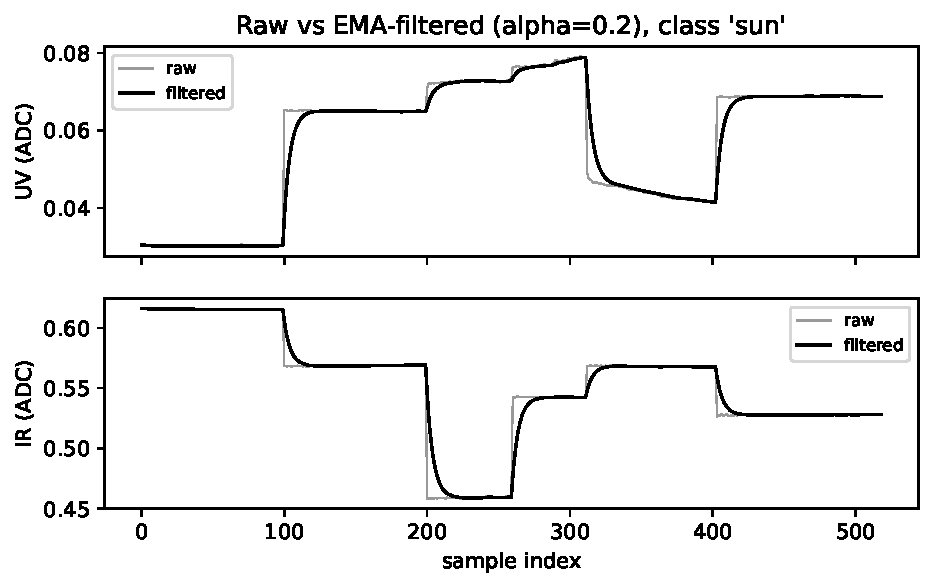
\includegraphics[width=\columnwidth]{filter_raw_vs_filtered.pdf}
\caption{Raw (grey) and EMA-filtered (black) UV and IR readings for one class, against
sample index. The filter suppresses short transients while preserving the class level
the classifier depends on.}
\label{fig:filter}
\end{figure}

\textbf{DBSCAN finds three of the four conditions without labels.}
Table~\ref{tab:dbscan} scores the discovered clusters against the true labels, which this
dataset, unlike Lab~3's, actually has. Sun is recovered perfectly: all 311 training points
in one cluster that contains nothing else. Incandescent (297) and LED (305) fall into the
same cluster. Shade splits three ways: 61 and 54 points in two shade-only clusters, and 169
inside the indoor cluster. Figure~\ref{fig:clusters} shows the same result spatially.

\begin{table}[!bt]
\centering
\caption{DBSCAN clusters versus true labels, training set, $\varepsilon=0.05$
($-1$ = noise).}
\label{tab:dbscan}
\begin{tabularx}{\linewidth}{@{}X r r r r r@{}}
\toprule
true label & $-1$ & 0 & 1 & 2 & 3 \\
\midrule
incandescent & 4 & 0 & 0 & 297 & 0 \\
LED & 0 & 0 & 0 & 305 & 0 \\
shade & 12 & 61 & 0 & 169 & 54 \\
sun & 0 & 0 & 311 & 0 & 0 \\
\midrule
assigned name & -- & shade & sun & indoor & shade \\
\bottomrule
\end{tabularx}
\end{table}

\begin{figure*}[t]
\centering
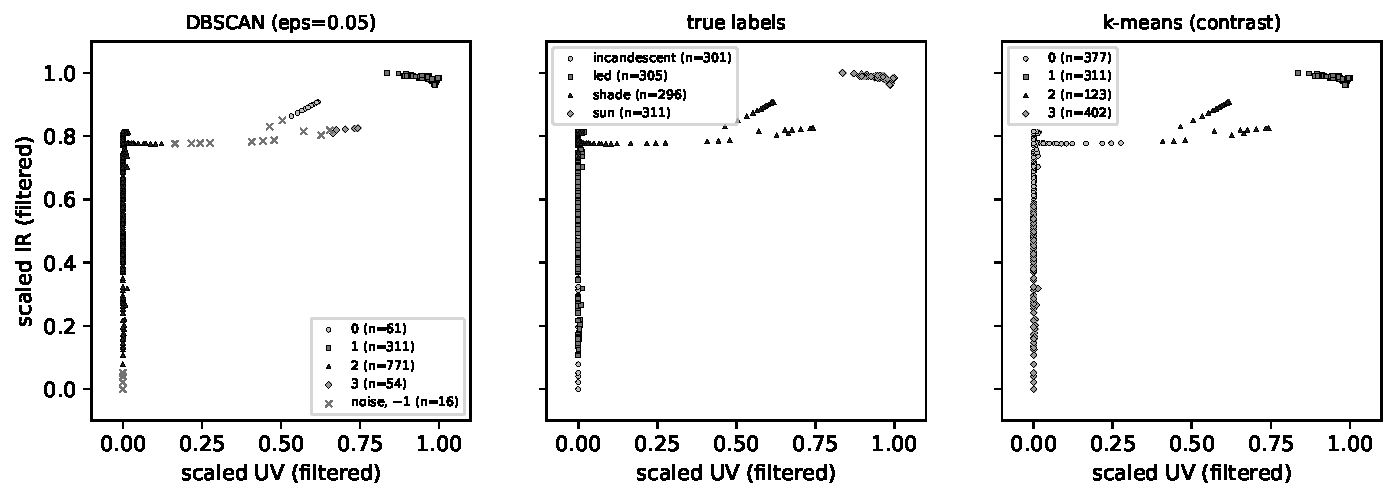
\includegraphics[width=0.95\textwidth]{clustered_space.pdf}
\caption{Training data in the scaled log-feature space, coloured by DBSCAN cluster (left),
true label (centre), and $k$-means with the same $k$ (right). Incandescent and LED occupy
the same region, so no clustering of these two features can separate them.}
\label{fig:clusters}
\end{figure*}

The disagreement is in the sensing, not the clustering. The IR channel read incandescent
light \emph{lower} than LED light (filtered $\approx$0.02 versus $\approx$0.1), the
opposite of their emission spectra, since incandescent bulbs emit far more infrared than
LEDs. With both at essentially zero UV, the two sources are not separable in this feature
space; the true-label panel of Figure~\ref{fig:clusters} shows it directly. DBSCAN's
answer is the correct one for the data it was given.

\textbf{The maps survive being stored as bytes.}
\todo{Insert Figure: class\_surfaces\_continuous.pdf beside class\_surfaces\_discretized.pdf,
and optionally total\_distribution.pdf.} Quantising each peak-normalised map to uint8 cost
a worst-case error of \todo{final value from DiscretizeSurfaces.py, $\approx$0.19}\% of
peak, within the theoretical bound $1/(2\cdot255)\approx0.196\%$. On the 405 held-out test
points the stored uint8 lookup reproduced the continuous KDE's decision for
\todo{final value from EvaluateTest.py}\% of them.

\textbf{The model costs what was predicted.} Table~\ref{tab:footprint} gives the footprint
for each storage format; we ship uint8. Table~\ref{tab:cost} compares prediction with
measurement. Flash was measured as the difference between the real firmware
(330{,}434\,B) and an otherwise identical build with a $G=2$ dummy table of 16\,bytes
(329{,}354\,B): 1080\,B against a predicted $1024-16=1008$\,B. The 72\,B excess is
attributable to segment alignment and to code that depends on the table's dimensions.
A first attempt with a $G=1$ dummy overstated the cost at 1336\,B, because with a single
cell the compiler removed the now-constant index arithmetic (about 244\,B of code); a cost
measurement must change only the component being measured. Global variables were
22{,}876\,B in both builds: the \texttt{const} table lives in flash and adds no SRAM.
Over 10{,}000 calls a classification took 0.658\,$\mu$s, about 160 cycles at 240\,MHz,
mostly the two \texttt{log1pf} calls. Acquisition, $2\times16$ ADC reads at 100\,$\mu$s
spacing, takes over 3\,ms, so the lookup is negligible at the 10\,Hz sample rate.

\begin{table}[!bt]
\centering
\caption{Model footprint by storage format ($K=4$, $G=16$), plus 16\,B of scaling bounds
in every case.}
\label{tab:footprint}
\begin{tabularx}{\linewidth}{@{}X r r r@{}}
\toprule
storage & B/cell & per class & all $K$ \\
\midrule
\texttt{uint8} & 1 & 256 & 1024 \\
\texttt{uint16} & 2 & 512 & 2048 \\
\texttt{float32} & 4 & 1024 & 4096 \\
\texttt{float64} & 8 & 2048 & 8192 \\
\bottomrule
\end{tabularx}
\end{table}

\begin{table}[!bt]
\centering
\caption{Predicted versus measured cost on the ESP32-S3.}
\label{tab:cost}
\begin{tabularx}{\linewidth}{@{}X r r@{}}
\toprule
quantity & predicted & measured \\
\midrule
table flash (vs.\ $G=2$ dummy) & 1008\,B & 1080\,B \\
table SRAM & 0\,B & 0\,B \\
byte reads per query & $K=4$ & 4 \\
time per query & -- & 0.658\,$\mu$s \\
\bottomrule
\end{tabularx}
\end{table}

\textbf{The device agrees with the desktop, and is right where the sensors allow.}
A held-out batch was recorded live, after training, with the device printing its filtered
readings and its decision. Recomputing each decision in Python from the same filtered values
gave \todo{agreement from CompareDevice.py}\% device--desktop agreement. Against the true
conditions (Table~\ref{tab:device}), the device was correct for incandescent (11/11, as
indoor), LED (11/11, as indoor), and sun (11/11), and wrong for all 9 shade readings,
which it reported as indoor: 33/42 = 78.6\% overall. The shade readings (IR $\approx$0.13,
UV 0) fall inside the LED range, the same overlap that put 169 shade training points into
the indoor cluster (Table~\ref{tab:dbscan}). The failure was predicted by the training
evidence, not discovered by surprise.

\begin{table}[!bt]
\centering
\caption{Live device predictions on the held-out batch.}
\label{tab:device}
\begin{tabularx}{\linewidth}{@{}X r r r@{}}
\toprule
true condition & indoor & shade & sun \\
\midrule
incandescent & 11 & 0 & 0 \\
LED & 11 & 0 & 0 \\
shade & 9 & 0 & 0 \\
sun & 0 & 0 & 11 \\
\bottomrule
\end{tabularx}
\end{table}

\textbf{Proof of concept.} Figure~\ref{fig:board} shows the wired board; a
\todo{30--60\,s} video of live classification is at \url{\todo{video link}}.

\begin{figure}[!bt]
\centering
% \includegraphics[width=\columnwidth]{board_photo.jpg}
\todo{Add your board photo here (uncomment the line above and fix the file name).}
\caption{The ESP32-S3 with the GUVA-S12SD UV module (GPIO7) and the IR photodiode divider
(GPIO8).}
\label{fig:board}
\end{figure}

% ------------------------------------------------------------------
\section{Limitations and remaining uncertainty}

The Lab~3 limitations about synthetic data and missing ground truth no longer apply: the
data is real and labelled. What the evidence does \emph{not} establish is the following.

\textbf{The IR channel does not separate the sources it was meant to separate.}
Incandescent read lower IR than LED, contrary to their spectra, so the two were merged
and the deployed classifier reports one ``indoor'' class. The likely causes are sensor
placement and distance during collection, or the photodiode's spectral response; we did
not isolate which.

\textbf{Shade is not reliably separable from indoor light.} One cluster in three shade
points fell into the indoor cluster during training, and every shade reading in the live
test was classified as indoor. Dim shade and an LED produce the same pair of readings on
these two sensors.

\textbf{Conditions drift between sessions.} Sun read IR $\approx$0.6 in training and
$\approx$0.40 in the live test, lowering the winning value from near 1 to 0.388. It still
cleared $\tau=0.12$, but a dimmer day could push sun towards the reject region.

\textbf{Training and live filtering differ in time.} Training data was logged one reading
per button press, so the offline EMA smoothed across presses seconds apart, whereas the
device samples at a fixed 10\,Hz. Steady light settles to the same filtered value either
way, but transients behave differently, and the filter's time constant is defined in
samples rather than in seconds.

\textbf{Small evidence base.} One sensor unit, one location, a few sessions, and a live
held-out batch of only 42 readings. The 78.6\% figure has a wide confidence interval and
says nothing about other windows, sensors, or seasons.

\textbf{Chosen, not derived, parameters.} $\tau=0.12$ and $\alpha=0.2$ were chosen rather
than optimised, and $h$ was set by the grid resolution because the validation criterion
degenerates on near-duplicate filtered data.

\textbf{What we would measure next.} First, re-collect incandescent and LED with the
photodiode aimed at the source at a fixed distance, and check that incandescent then reads
higher IR, which would test whether the merge is a setup error. Second, log at a fixed
sample rate equal to the deployed one, across several days and times, to measure drift and
remove the filter mismatch. Third, record a held-out batch of at least 100 readings per
condition so the accuracy figure means something. If the IR fix separates the indoor
sources, the pipeline needs no change: DBSCAN would find a fifth cluster and the table
would grow by 256 bytes.

\end{document}
